% CHAPTER 5.4: COPILOT --- CROSS-PAGE MULTI-AGENT INTELLIGENT DISPATCHER
% ======================================================================
\subsection{Copilot --- A Unified Intelligent Dispatcher Above the Three Agents}

The three agents described in Sections 5.1--5.3 each solve a specific domain problem, but from the user's perspective, they still require knowing \textit{which} agent to use before typing a question. A bank employee asking ``Which meeting rooms are free this afternoon?'', ``How many pending transactions are there?'', or ``Which policy clause explains this approval rule?'' should not need to understand whether the request belongs to the Tool Agent, Code Agent, or RAG Agent. The Copilot solves this by sitting above all three agents as a single natural language entry point: the user says what they need, and the Copilot figures out where it should go.

\subsection{Design Rationale}

The Copilot is not a fourth agent with its own domain capability. It is a \textbf{dispatcher} --- its only job is to understand the user's intent, route the request to the right agent, and present the result back in a unified chat interface. This design follows a simple principle: the platform has exactly one text box the user needs to care about, and it works across every page.

Table \ref{tab:copilot-vs-agents} summarizes the Copilot's position relative to the three agents.

\begin{table}[H]
\centering
\small\singlespacing
\caption{Copilot vs. Three Domain Agents --- Role Comparison}
\label{tab:copilot-vs-agents}
\begin{tabularx}{\textwidth}{>{\RaggedRight\arraybackslash}X>{\RaggedRight\arraybackslash}p{0.42\textwidth}>{\RaggedRight\arraybackslash}p{0.34\textwidth}}
\toprule
& \textbf{Three Domain Agents} & \textbf{Copilot} \\
\midrule
Role & Execute domain-specific tasks (SQL, retrieval, tools) & Classify intent and dispatch \\
Input & Already-routed request with known type & Raw natural language, any topic \\
Output & Domain result (SQL rows, document excerpts, room lists) & Dispatch decision + agent result in chat \\
Scope & One agent = one capability & Cross-agent, cross-page \\
User interaction & Page-specific UI (tables, maps, panels) & Floating chat widget, always accessible \\
\bottomrule
\end{tabularx}
\end{table}

\subsection{Architecture Overview}

The Copilot spans three layers of the platform. On the frontend, a Vue 3 floating widget (CopilotWidget.vue) renders inside the global MainLayout, making it accessible from every page. On the backend, a Python Flask intent classifier (port 8090, shared with the Code Agent's inference server) performs the core dispatch logic. Between them, the Task Service provides asynchronous execution and WebSocket-based progress streaming for long-running agent calls.

Figure \ref{fig:copilot-flow} shows how a user query flows through the Copilot system.

\begin{figure}[H]
\centering
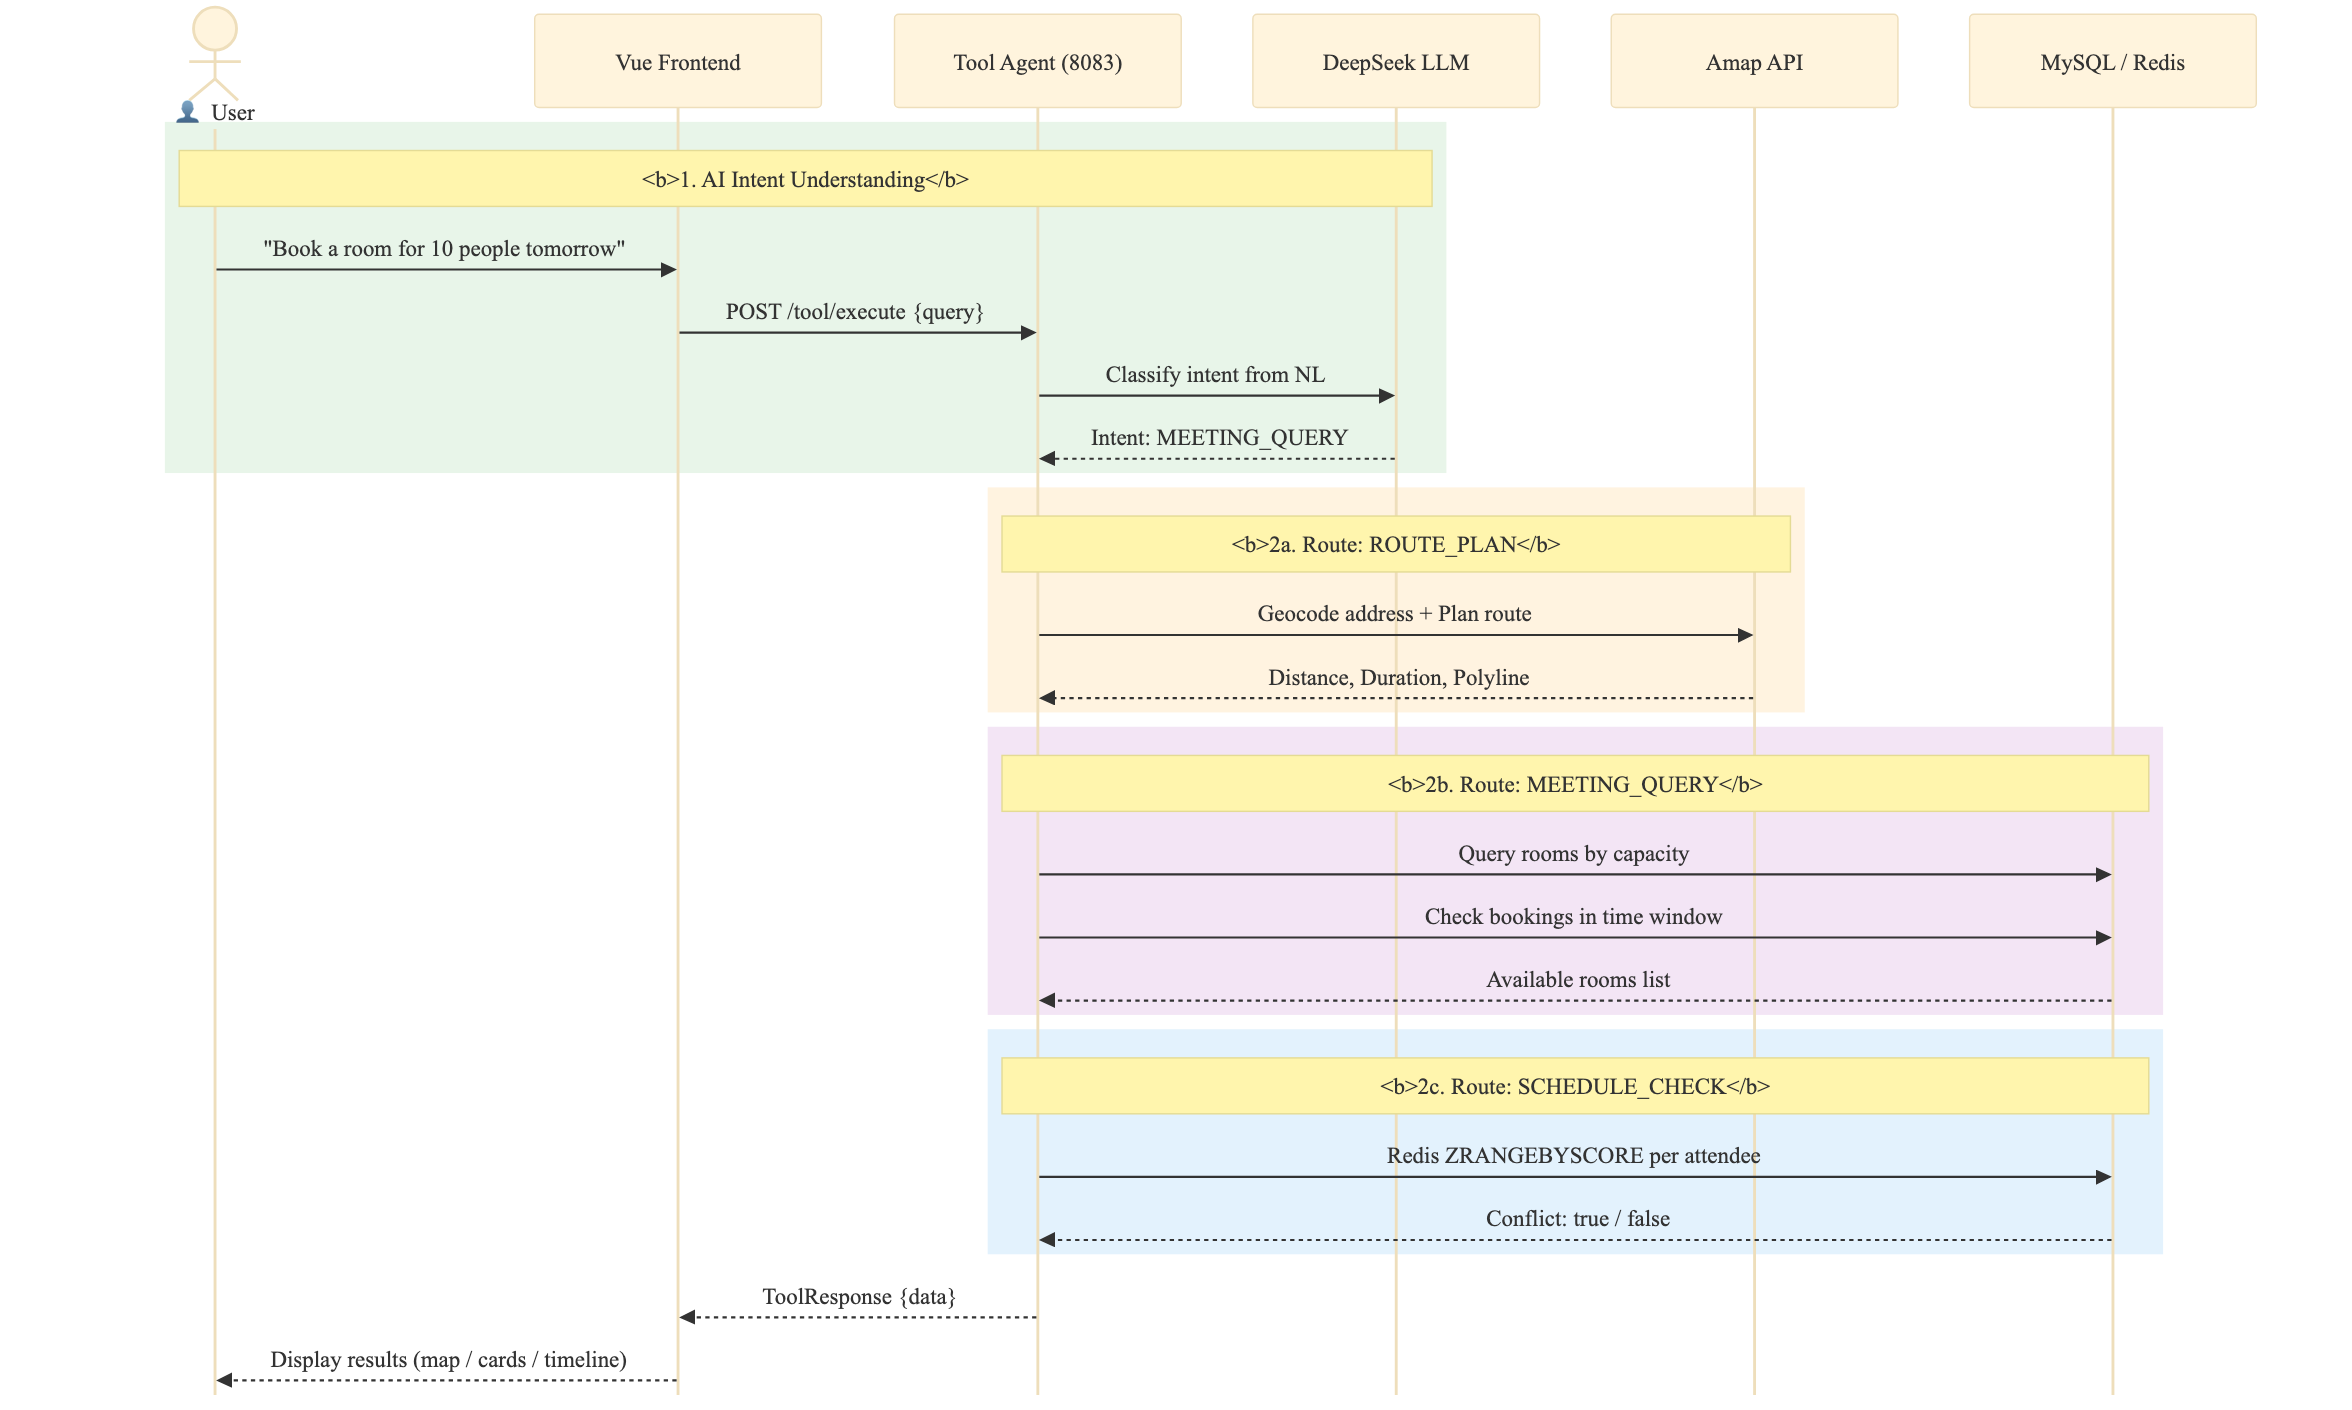
\includegraphics[width=0.92\textwidth]{figures/fig05_tool_agent_sequence.png}
\caption{Copilot Query Flow --- From Natural Language to Agent Execution}
\label{fig:copilot-flow}
\end{figure}

The flow has four stages. First, the user types a question into the Copilot widget. Second, the widget sends the question to \texttt{POST /api/dashboard/route}, which the Gateway rewrites to \texttt{/route} on the Python Flask server. Third, Flask runs a three-tier classification pipeline and returns an intent label. Fourth, the frontend dispatches based on the label: chat replies are shown inline, while domain tasks (TOOL, RAG) are submitted to the Task Service for asynchronous execution with progress streaming.

\subsection{Three-Tier Intent Classification}

The Python Flask \texttt{/route} endpoint is the Copilot's brain. It implements a three-tier classification strategy that balances cost, latency, and accuracy, shown in Table \ref{tab:three-tier}.

\begin{table}[H]
\centering
\small\singlespacing
\caption{Three-Tier Intent Classification Strategy}
\label{tab:three-tier}
\begin{tabularx}{\textwidth}{>{\RaggedRight\arraybackslash}p{0.12\textwidth}>{\RaggedRight\arraybackslash}p{0.26\textwidth}>{\RaggedRight\arraybackslash}p{0.38\textwidth}>{\RaggedRight\arraybackslash}p{0.24\textwidth}}
\toprule
\textbf{Tier} & \textbf{Mechanism} & \textbf{What It Catches} & \textbf{Cost} \\
\midrule
Tier 1 & Pattern blocklist (40+ regex rules) & Jailbreak attempts, non-banking topics, prompt injection & Zero (no API call) \\
Tier 2 & Keyword greeting match & ``Hello'', ``What can you do'', simple greeting phrases & Zero \\
Tier 3a & LLM classification (temperature=0.1, max\_tokens=10) & CODE, TOOL, RAG, CHAT, CLARIFY, SETTINGS & $\sim$10 tokens per query \\
Tier 3b & Keyword fallback (LLM unavailable) & Same six categories, lower accuracy & Zero \\
\bottomrule
\end{tabularx}
\end{table}

Tier 1 acts as a pre-screening safety net. Before any LLM call is made, the user's input is checked against a hardcoded list of approximately 40 blocked patterns. These cover jailbreak prompts (e.g., ``ignore previous instructions''), role-play attempts (``pretend you are a hacker''), code injection, and entirely off-topic requests (jokes, recipes, gaming). Blocked queries are caught instantly and receive a polite refusal without consuming any API tokens.

Tier 2 catches simple greetings. If the user says ``Hello'' or ``What can you do?'' or the Chinese equivalent, the system responds with a friendly introduction listing the four capabilities (database queries, policy Q\&A, meeting and schedule tools, route planning) --- again with zero LLM cost.

Tier 3a is the core classification layer. The user's question is sent to the LLM with a system prompt defining six intent categories:

\begin{itemize}
  \item \textbf{CODE}: Database queries, statistics, data lookups --- anything that translates to SQL.
  \item \textbf{TOOL}: Meeting room booking, schedule conflict checking, route planning.
  \item \textbf{RAG}: Policy documents, regulations, concept definitions, compliance guidelines.
  \item \textbf{CLARIFY}: The user wants to book a room or plan a route, but has not provided enough parameters (e.g., no time specified for a meeting, no destination for a route).
  \item \textbf{SETTINGS}: Password changes, profile configuration.
  \item \textbf{CHAT}: Greetings, casual conversation, or anything outside the platform's scope.
\end{itemize}

The LLM is configured with temperature 0.1 and max\_tokens 10 --- the response is a single word, not a sentence. This keeps classification deterministic and cheap. For CLARIFY and CHAT intents, a second LLM call generates a conversational reply with appropriate follow-up questions or explanations.

Tier 3b activates only when the LLM API is unreachable. A pure keyword-matching fallback scans for terms associated with each intent --- for CODE: terms related to databases, statistics, and data queries; for TOOL: terms related to meeting rooms, bookings, and schedules; and for RAG: terms related to policies, regulations, manuals, document search, citations, and knowledge-base questions. If no keyword group is matched, the classifier defaults to RAG because document Q\&A is the safest read-only fallback. This ensures the Copilot degrades gracefully rather than failing completely.

\subsection{Frontend Dispatch and User Experience}

After the intent is classified, the frontend widget takes over with type-specific handling, summarized in Table \ref{tab:intent-dispatch}.

\begin{table}[H]
\centering
\small\singlespacing
\caption{Intent Dispatch --- Frontend Behavior by Classification Result}
\label{tab:intent-dispatch}
\begin{tabularx}{\textwidth}{>{\RaggedRight\arraybackslash}p{0.16\textwidth}>{\RaggedRight\arraybackslash}p{0.40\textwidth}>{\RaggedRight\arraybackslash}X}
\toprule
\textbf{Intent} & \textbf{Widget Action} & \textbf{User Sees} \\
\midrule
CHAT & Display reply text directly in chat bubble & The LLM's conversational response \\
CLARIFY & Save context, ask follow-up question & ``Could you tell me what time you need the room?'' --- next user message prepends saved context \\
SETTINGS & Navigate to settings page & The settings form \\
CODE & Fire custom event, navigate to /app/code & The Code Agent page with the question pre-filled \\
TOOL & Submit task $\rightarrow$ WebSocket progress $\rightarrow$ result card & Animated processing bar with rotating status messages, then a result card (room list, conflict report, or route map) \\
RAG & Submit task $\rightarrow$ WebSocket progress $\rightarrow$ result card & A citation card with document titles, similarity scores, and security badges \\
\bottomrule
\end{tabularx}
\end{table}

The Copilot widget itself is a floating component: a 52px circular icon button fixed to the bottom-right corner of every page. When clicked, it expands into a 440$\times$620px chat panel with a morphing animation. This design means the user never leaves their current page to ask a question --- the Copilot comes to them.

During agent execution, the input area is replaced by an animated processing bar. A pulsing blue dot, a water-ripple effect radiating from the input, and a set of status messages (``Analyzing your request...'', ``Identifying intent...'', ``Routing to the right agent...'', ``Processing with AI model...'', ``Gathering results...'', ``Almost there...'') rotated every 1.5 seconds give the user continuous feedback. A live elapsed-time counter ticks every 100ms, so the user knows the system has not frozen.

When a task completes, the raw JSON output from the agent is transformed into a human-readable result card. Meeting queries show room names with colored availability dots, capacity badges, and location. Route plans show distance, duration, and traffic status. RAG answers show citation counts, blocked document counts, and a ``View details'' link. Conflict detections show either a green all-clear or an amber warning with the conflicting schedule details.

Session history is persisted in the browser's localStorage under the key prefix \texttt{copilot\_session\_}, with a session index limited to 20 entries. Users can review past conversations or start a fresh session from the history panel.

\subsection{Multi-Turn Clarification}

The CLARIFY intent enables a simple but effective multi-turn dialogue pattern. If a user types ``Book a meeting room,'' the classifier recognizes that critical parameters are missing and returns CLARIFY. The widget saves the original query into a \texttt{sessionContextQuery} variable and displays the LLM's follow-up question (e.g., ``What time and how many people?''). When the user replies ``Three o'clock, five people,'' the widget prepends the saved context to form a combined query --- ``Book a meeting room [context: Three o'clock, five people]'' --- and re-classifies. This time, with all parameters present, the classifier returns TOOL and the request proceeds to the Tool Agent.

\subsection{Cross-Page Communication}

Because the Copilot widget is rendered once in MainLayout and persists across page navigation, it needs a mechanism to deliver agent results to whichever page the user is currently viewing. Two channels handle this:

\begin{enumerate}
  \item \textbf{Browser Custom Events}: The widget dispatches \texttt{CustomEvent} objects on the \texttt{window} object --- \texttt{copilot-tool-result} for Tool Agent results, \texttt{copilot-code-query} for Code Agent queries, and \texttt{copilot-rag-query} for RAG Agent questions and citation-based answers. Target page components listen for these events and react accordingly.
  \item \textbf{localStorage}: As a safety net for pages that mount \textit{after} the event was dispatched (e.g., the widget navigated to a new page before the subscribing component existed), tool results, code queries, and RAG query payloads are also written to localStorage keys. The target page checks these keys on mount and processes any pending result.
\end{enumerate}

\subsection{Second-Level Intent Classification in the Tool Agent}

When the Copilot classifies a query as TOOL, the Task Service forwards it to the Tool Agent's \texttt{/tool/execute} endpoint with \texttt{toolType: "AI"}. At this point, a second classification happens inside the Tool Agent itself. The \texttt{handleAiIntent()} method sends the query to DeepSeek with a system prompt asking it to distinguish between three sub-intents: MEETING\_QUERY, SCHEDULE\_CHECK, and ROUTE\_PLAN. The LLM returns a JSON object with the sub-intent and extracted parameters, which the Tool Agent uses to call the appropriate handler.

This two-level classification --- Copilot first decides \textit{which agent}, then the Tool Agent decides \textit{which tool} --- keeps each classifier's job simple. The Copilot's classifier only needs to distinguish broad domains; the Tool Agent's classifier only needs to distinguish between its own three tools. Neither classifier needs to understand the full complexity of the entire platform.

\subsection{AI Provider Configuration Unification}

Before the Copilot was introduced, each agent that called an LLM managed its own API key and endpoint configuration independently. The Tool Agent's DeepSeek service had its own \texttt{application.yml} block; the Python inference server read from a separate \texttt{ds\_config.json} file; the RAG Agent had a third set of environment variables.

The Copilot unified all AI provider configuration under the user-service's \texttt{SystemConfigController}. A single admin UI (Settings page) accepts the provider name, base URL, model name, and API key. The key is AES-256 encrypted before storage in MySQL and cached in Redis under \texttt{sys:config:ai\_provider}. Two REST endpoints serve the configuration:

\begin{itemize}
  \item \texttt{GET /user/config/ai-provider} (public): Returns provider, base URL, and model --- the API key is stripped for security. Used by the frontend to display the current model.
  \item \texttt{GET /user/config/ai-provider/internal} (internal, not exposed through the Gateway): Returns the full configuration including the decrypted API key. Called by the Python Flask classifier, the Tool Agent's DeepSeekService, and the RAG Agent. Because this endpoint is not routed through the Gateway, it is only reachable from within the Docker internal network.
\end{itemize}

With this unification, changing the LLM provider for the entire platform requires updating a single form --- no configuration files to edit, no service restarts.

\newpage

% ======================================================================
